\graphicspath{{figures/dynamic/}}

\chapter{考虑龙卷风平移的动态响应分析}

第\ref{chapter:static}章忽略了龙卷风平移运动的影响,
分别在\SI{0}{\degree}、\SI{45}{\degree}和\SI{90}{\degree}工况下进行静力非线性分析。
本章考虑龙卷风平移运动的影响,假定其移动轨迹后计算输电塔结构各节点荷载时程,
进行动力时程分析,分析其动态响应。

\section{动态龙卷风模型}

根据第\ref{sec:tower-fea}建立整体坐标系,如图\ref{fig:tower-tornado-cs}所示。
龙卷风相应于输电塔结构做平移运动的示意图见图\ref{fig:tornado-path}所示。
\begin{figure}[!htpb]
	\centering
	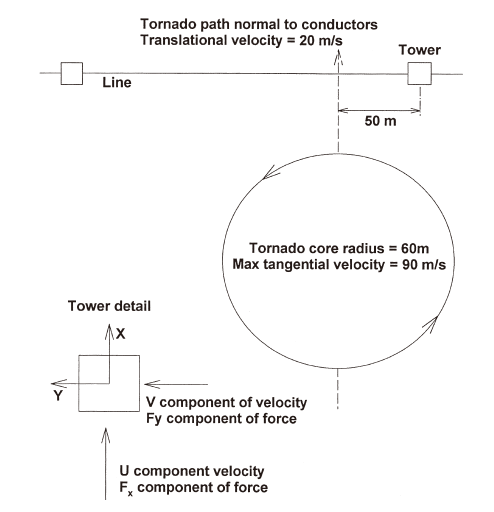
\includegraphics[width=0.6 \textwidth]{tornado-path.png}
	\caption{龙卷风相应于输电塔做平移运动的示意图}
	\label{fig:tornado-path}
\end{figure}

\subsection{龙卷风路径}

假定龙卷风核心在地面上做匀速直线运动,描述其路径的关键参数为核心初始位置和运动速度。

为了使得初始时刻输电塔结构所受龙卷风荷载较小,需要将龙卷风核心初始位置设置在距离输电塔较远的地方。
若初始时刻龙卷风核心距离输电塔很近,结构会受到量值很大的突加荷载的影响,与实际情况不符。
初始位置在整体坐标系中的位置记为$\left(x^T_{0},y^T_{0}\right)$。

关于龙卷风的平移速度在第\ref{sec:tornado-cha}节已有介绍,
我国《三十万千瓦压水堆核电厂安全重要土建结构抗龙卷风设计规定》中A类龙卷风平移速度为\SI{22.4}{m/s},
文献\cite{savory2001modelling}\cite{hamada2011behaviour}中选用龙卷风平移速度为\SI{20.0}{m/s},
二者差别较小,本文为计算简便选用$v^T=\SI{20.0}{m/s}$。
确定龙卷风路径还需龙卷风平移速度的方向,设平移速度相对于输电线、即$X$轴正向的夹角为$\theta^T$。

综上,龙卷风运动轨迹$\left(x^T(t),y^T(t)\right)$可表示为:
\begin{equation}
	\begin{cases}
		x^T(t) = x^T_0 + \left(v^T\cos{\theta^T}\right)t \\
		y^T(t) = y^T_0 + \left(v^T\sin{\theta^T}\right)t 
	\end{cases}
\end{equation}
龙卷风的平移运动引起了龙卷风核心相对输电塔位置$\left(x^T(t),y^T(t)\right)$随时间变化,
进而使得输电塔受到了随龙卷风位置变化的荷载时程,需进行动力时程分析计算结构响应。

本文假设龙卷风风场结构不随时间变化(实际中龙卷风会随其运动衰减,本文忽略这一现象),
即采用第\ref{sec:full-tornado}中模拟的足尺龙卷风风场作为任一时刻动态龙卷风的风场。

\section{动态龙卷风风速及荷载时程}

在任意时刻$t$,利用第\ref{sec:static-code}节中规范方法施加该时刻的龙卷风荷载。
由于第\ref{sec:static-code}节已编制了计算龙卷风荷载并施加到输电塔结构的APDL程序,
在动力分析中,改变龙卷风核心相应于输电塔中心的极坐标$(R,\theta)$(见第\ref{sec:d-polor}节),
调用龙卷风荷载施加子程序,即可完成动态荷载施加过程。

\subsection{典型龙卷风运动工况}

龙卷风平移运动的两种典型工况见图\ref{fig:dynamic-case1}和图\ref{fig:dynamic-case2}。
图\ref{fig:dynamic-case1}中龙卷风运动路径平行于输电线,下文简称为龙卷风平行运动工况;
图\ref{fig:dynamic-case2}中龙卷风运动路径垂直于输电线,下文简称为龙卷风垂直运动工况。

\begin{figure}[!htpb]
    \centering
    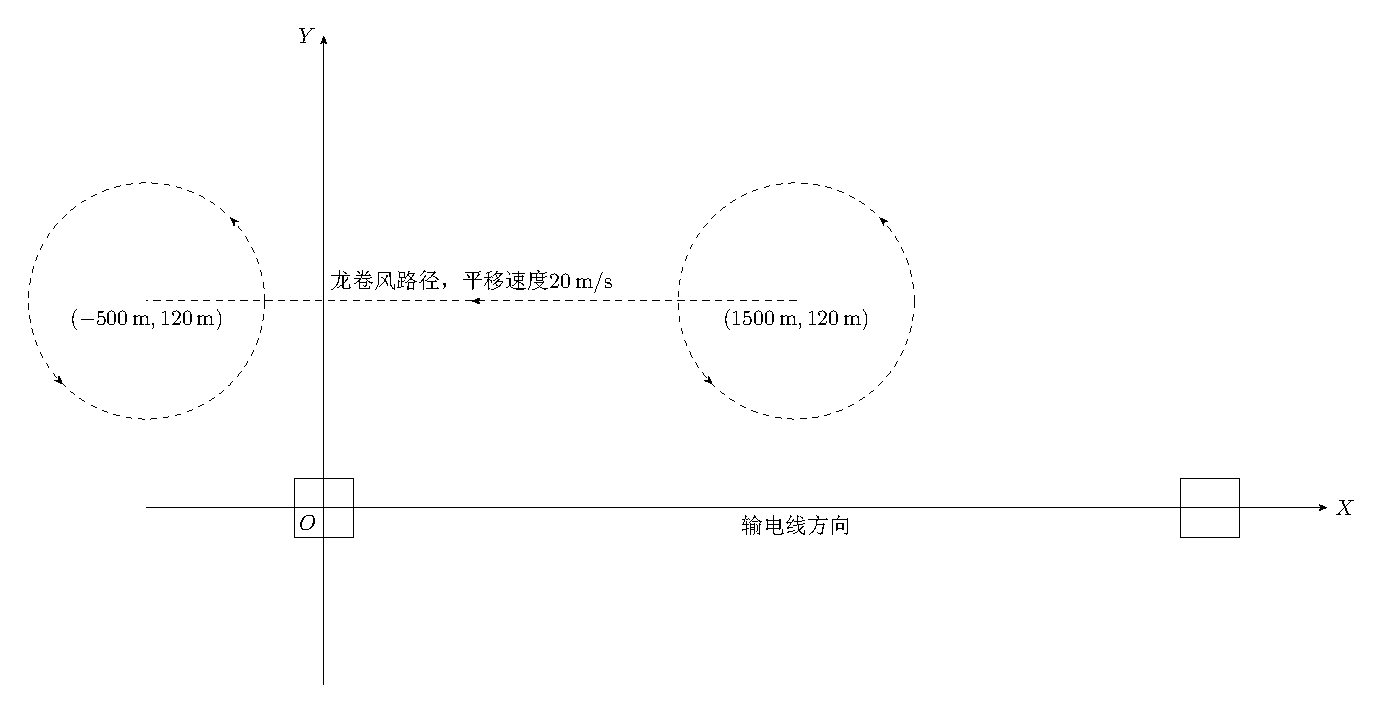
\includegraphics[width=\textwidth]{dynamic-case1.pdf}
    \caption{龙卷风平行运动工况}
    \label{fig:dynamic-case1}
\end{figure}
\begin{figure}[!htpb]
    \centering
    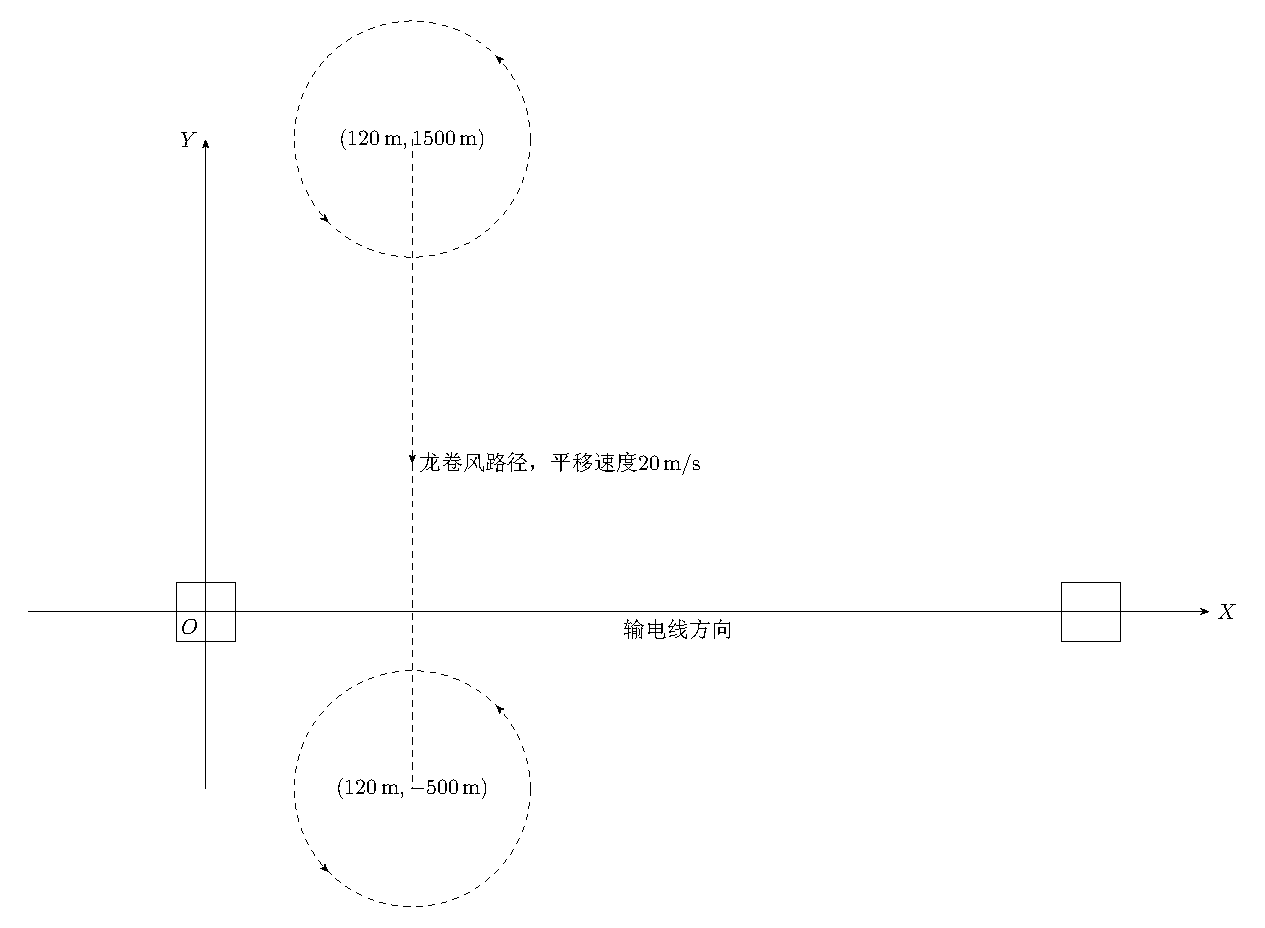
\includegraphics[width=\textwidth]{dynamic-case2.pdf}
    \caption{龙卷风垂直运动工况}
    \label{fig:dynamic-case2}
\end{figure}

平行运动工况(图\ref{fig:dynamic-case1})中,
龙卷风核心初始位置选为$x_0^T=\SI{1500}{m}$,$y_0^T=\SI{120}{m}$;
平移速度$v^T=\SI{20.0}{m/s}$,$\theta^T=\pi$。
满足初始时刻龙卷风距离输电塔较远,龙卷风荷载较小,
且在运动过程二者距离取得龙卷风核心半径$r_c=\SI{120}{m}$,受到龙卷风荷载较大。

类似选取垂直运动工况(图\ref{fig:dynamic-case2})的参数,
龙卷风核心初始位置选为$x_0^T=\SI{120}{m}$,$y_0^T=\SI{1500}{m}$;
平移速度$v^T=\SI{20.0}{m/s}$,$\theta^T=-\frac{1}{2}\pi$。

\subsection{动态龙卷风风速时程}

随着龙卷风移动位置的变化,输电塔结构各节点受到风速时程的作用。
现选取塔顶节点,平行工况和垂直工况时塔顶节点风速时程分别如图\ref{fig:velo_case1}、图\ref{fig:velo_case2}所示。
\begin{figure}[!htpb]
    \centering
    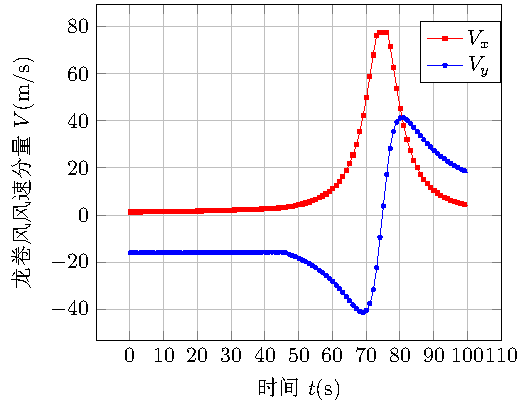
\includegraphics[width=0.6\textwidth]{velo_case1.pdf}
    \caption{龙卷风运动平行工况塔顶节点风速时程}
    \label{fig:velo_case1}
\end{figure}
\begin{figure}[!htpb]
    \centering
    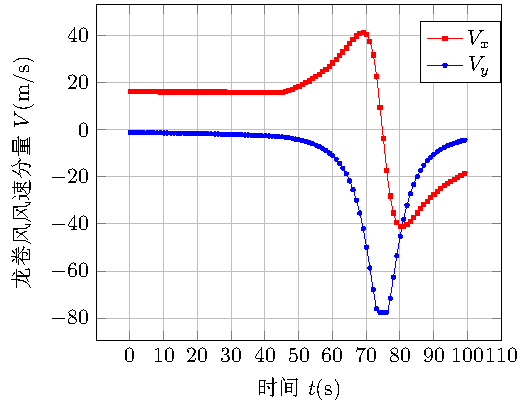
\includegraphics[width=0.6\textwidth]{velo_case2.pdf}
    \caption{龙卷风运动垂直工况塔顶节点风速时程}
    \label{fig:velo_case2}
\end{figure}

\subsection{动态龙卷风荷载时程}

在龙卷风移动过程中,任一时刻确定龙卷风位置后,
根据规范方法(第\ref{sec:static-code}节)计算输电塔结构受到的龙卷风荷载。
并将结构有限元模型所有节点受到的龙卷风荷载在$X$和$Y$轴的分量进行求和,
绘制龙卷风荷载分量合力的时程曲线,如图\ref{fig:sum_f_case1}和\ref{fig:sum_f_case2}所示。
\begin{figure}[!htpb]
    \centering
    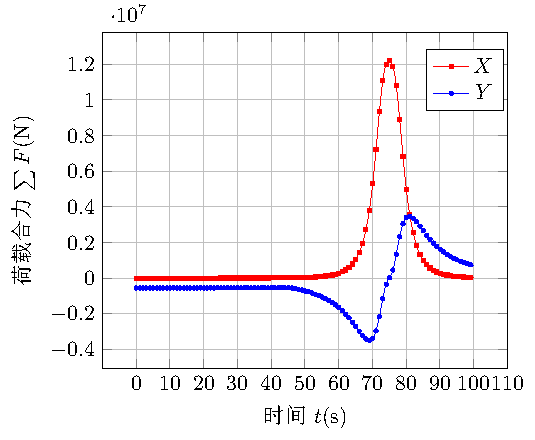
\includegraphics[width=0.6\textwidth]{sum_f_case1.pdf}
    \caption{龙卷风运动平行工况荷载分量合力时程}
    \label{fig:sum_f_case1}
\end{figure}
\begin{figure}[!htpb]
    \centering
    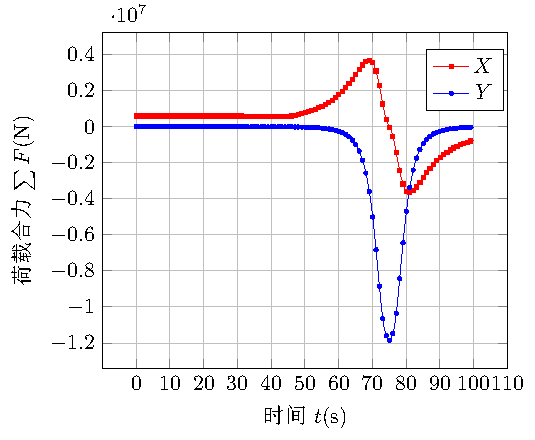
\includegraphics[width=0.6\textwidth]{sum_f_case2.pdf}
    \caption{龙卷风运动垂直工况荷载分量合力时程}
    \label{fig:sum_f_case2}
\end{figure}

\section{输电塔结构动力时程分析}

对输电塔进行风荷载动态响应分析,常采用时程分析方法,
即将动态龙卷风荷载施加到结构上,利用数值方法求解动力运动方程,
可全面了解结构在龙卷风动态荷载作用时间内的动力响应状况,求解精度较高。
本文采用时程分析方法分析输电塔结构在龙卷风作用下的动态响应。

由于时程分析方法计算量较大,故本节不考虑输电塔结构材料非线性和几何非线性的影响。
由于输电线与塔结构的耦合效应机理复杂,本文忽略这一效应的影响。
时间步长初选为\SI{0.10}{s},
并进行时间步长的敏感性分析,发现当时间步长减小为\SI{0.05}{s}时结构动态响应差别较小。
这说明\SI{0.10}{s}的时间步长是足够精确的。

\subsection{动力方程及其求解}

输电塔结构在考虑移动效应的龙卷风荷载时程作用下的动力方程为:
\begin{equation}\label{eqn:dynamic}
    \bm{M}\ddot{\bm{u}}+\bm{C}\dot{\bm{u}}+\bm{K}\bm{u} = \bm{F}(t)
\end{equation}
式中:$\bm{M}$、$\bm{C}$和$\bm{K}$分别为输电塔结构总体质量矩阵、阻尼矩阵及刚度矩阵;
$\ddot{\bm{u}}$、$\dot{\bm{u}}$和$\bm{u}$分别为节点的加速度、速度及位移向量;
$\bm{F}$为输电塔受到的龙卷风荷载时程。

对结构的时程分析一般采用逐步积分方法。
从积分格式的形式上可划分为隐式方法与显式方法;
从计算格式的稳定性上可划分为无条件稳定方法与条件稳定方法。
评价逐步积分方法的优劣包括稳定性、精度、高频能耗性及幅值超越性。
其中稳定性占有重要地位。
无条件稳定的逐步积分方法在应用时,其计算时间步长不受方法本身所控制,而仅由计算精度要求确定;
条件稳定的逐步积分方法的计算时间步长,不但要受计算精度要求的控制,而且还受其稳定条件的限制。
隐式逐步积分方法与显示方法的区别在于计算格式所形成的线性方程组的耦联与否。
显式方法一般为条件稳定,故只在某些领域如离散网格中波动的研究中采用。
隐式逐步积分方法的研究成果较多,在结构计算中得到应用的有常平均加速度方法、Newmark法和Wilson-$\mathrm{\theta}$法等。

本文采用隐式的直接积分方法Newmark法对输电塔体系进行动力时程分析求解。

Newmark法假设$t+\Delta t$时刻的速度和位移为:
\begin{equation}\label{eqn:newmark-v}
  \dot{\bm{u}}_{t+\Delta t}=\dot{\bm{u}}_{t}+\left[(1-\gamma)\ddot{\bm{u}}_t+\gamma \ddot{\bm{u}}_{t+\Delta t}\right] \quad(0 \leq \gamma \leq 1)
\end{equation}
\begin{equation}\label{eqn:newmark-a}
  \bm{u}_{t+\Delta t}=\bm{u}_t + \dot{\bm{u}}_{t} \Delta t+\frac{1}{2}\left[\left(\frac{1}{2}-\beta\right)\ddot{\bm{u}}_{t}+\beta\ddot{\bm{u}}_{t+\Delta t}\right] \Delta t^2 \quad \left(0 \leq \beta \leq \frac{1}{2}\right)
\end{equation}
由式\eqref{eqn:newmark-a}可以解得:
\begin{equation}\label{eqn:newmark-a2}
  \ddot{\bm{u}}_{t+\Delta t}=\frac{1}{\beta \Delta t^2} \left(\bm{u}_{t+\Delta t}-\bm{u}_{t}\right)-\frac{1}{\beta \Delta t} \dot{\bm{u}}_t - \left(\frac{1}{2\beta}-1\right) \ddot{\bm{u}}_t
\end{equation}
将式\eqref{eqn:newmark-a2}代入式\eqref{eqn:newmark-v},然后共同代入式\eqref{eqn:dynamic},
则得到从$\bm{u}_t$、$\dot{\bm{u}}_t$和$\ddot{\bm{u}}_t$计算$\bm{u}_{t+\Delta t}$的两步递推公式为:
\begin{equation}
\begin{split}
  \left(\bm{K}+\frac{1}{\beta \Delta t^2} \bm{M} + \frac{\gamma}{\beta \Delta t} \bm{C} \right) \bm{u}_{t+\Delta t} = \bm{F}_{t+\Delta t} + \\
  \bm{M} \left[ \frac{1}{\beta \Delta t^2} \bm{u}_t + \frac{1}{\beta \Delta t} \dot{\bm{u}}_t + \left(\frac{1}{2\beta} - 1 \right)\ddot{\bm{u}}_t\right] + \\
  \bm{C} \left[ \frac{\gamma}{\beta \Delta t} \bm{u}_t + \left(\frac{\gamma}{\beta} - 1 \right) \dot{\bm{u}}_t + \left(\frac{\gamma}{2\beta} - 1 \right) \Delta t \ddot{\bm{u}}_t\right]
\end{split}
\end{equation}

Newmark方法中,当参数$\gamma\geq 0.5$,$\beta \geq 0.25\left(0.5 + \gamma\right)^2$时,
算法是无条件稳定的,即时间步长$\Delta t$的大小不影响解的稳定性。


\subsection{输电塔结构的阻尼}

阻尼能耗散动力系统能量,使自由振动的振幅随时间衰减。
影响结构动力响应的阻尼主要有粘性阻尼、滞后阻尼、库伦阻尼等\cite{chopra2007dynamic}。
结构动力分析的阻尼通常足够小,不考虑其实际来源,将其看做粘性阻尼,可足够精确模拟阻尼对结构的影响。

描述粘性阻尼的方法通常称为比例阻力(又称Rayleigh阻尼)和模态阻尼。
在使用直接积分法求解结构动力方程时,通常采用比例阻尼。
比例阻尼矩阵定义为结构总体质量矩阵和刚度矩阵的线性组合,即:
\begin{equation}
  \bm{C} = \alpha_1 \bm{M} + \alpha_2 \bm{K}
\end{equation}
式中:$\alpha_1$和$\alpha_2$分别为质量和刚度阻尼系数。
具体表达式为:
\begin{equation}
    \begin{cases}
        \alpha_1 = \frac{2\left(\zeta_i\omega_j-\zeta_j \omega_i\right)}{\omega_j^2-\omega_i^2} \omega_i \omega_j \\
        \alpha_2 = \frac{2\left(\zeta_j \omega_j-\zeta_i \omega_i\right)}{\omega_j^2-\omega_i^2} 
    \end{cases}
\end{equation}
其中$\omega_i$、$\omega_j$分别为结构的第$i$、$j$阶固有频率;
$\zeta_i$、$\zeta_j$分别为结构的第$i$、$j$阶振型的阻尼比。
通常工程计算中取前两阶。

在计算大跨越输电塔的结构阻尼时,
文献\cite{wong2009guidelines}\cite{loredo2003influence}\cite{madugula2001dynamic}\cite{ostendorp1997damping}
建议只考虑其第一阶振型及频率,
且不考虑质量矩阵对阻尼的影响,
即取$\alpha_1=0$,$\alpha_2=2\zeta/\omega$,
取结构的阻尼比$\zeta=0.04$\cite{loredo2003influence},
由此可计算处结构的阻尼矩阵。

\subsection{输电塔动态响应结果}

龙卷风动态荷载作用下,输电塔塔顶节点动态位移响应见图\ref{fig:disp_top_case1}和图\ref{fig:disp_top_case2}所示。
\begin{figure}[!htpb]
    \centering
    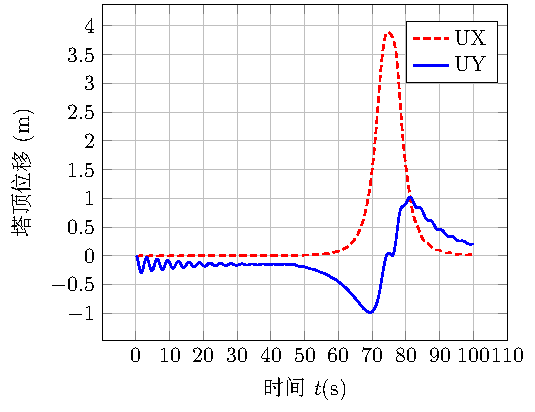
\includegraphics[width=0.6\textwidth]{disp_top_case1.pdf}
    \caption{龙卷风运动平行工况塔顶节点位移响应时程}
    \label{fig:disp_top_case1}
\end{figure}
\begin{figure}[!htpb]
    \centering
    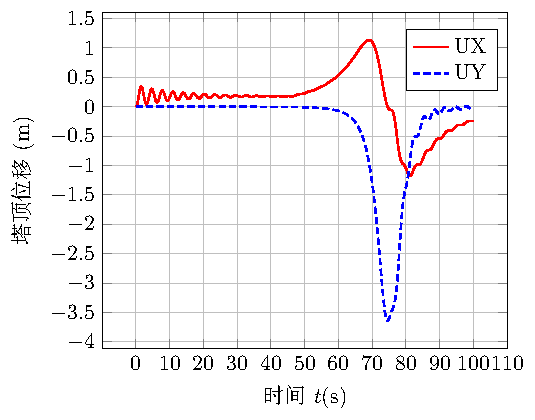
\includegraphics[width=0.6\textwidth]{disp_top_case2.pdf}
    \caption{龙卷风运动垂直工况塔顶节点位移响应时程}
    \label{fig:disp_top_case2}
\end{figure}
